\documentclass{article}
\usepackage{txfonts}
\usepackage{booktabs}
\usepackage{color}
\usepackage{bussproofs}
\usepackage{graphicx}
\usepackage{pifont}
\usepackage{qtree}
\usepackage{tikz}

\newenvironment{scprooftree}[1]%
{\gdef\scalefactor{#1}\begin{center}\proofSkipAmount \leavevmode}%
{\scalebox{\scalefactor}{\DisplayProof}\proofSkipAmount \end{center} }

\begin{document}
\author{Jappie Klooster}
\title{On proving things}
\maketitle

\section{Prove $R_k$}
Prove that the rule $R_k$ of the calculus $GKC_k$ is sound with respect to
Kripke models: If $I(\Gamma \Rightarrow A)$ holds in all Kripke models, then
so does $I(\Pi, \Box \Gamma \Rightarrow \Box A, \Delta)$

\begin{prooftree}
	\AxiomC{$\Gamma \Rightarrow A$}
	\RightLabel{$R_k$}
	\UnaryInfC{$\Pi, \Box \Gamma \Rightarrow \Box A, \Delta$}
\end{prooftree}

Take an arbitrary kripke model $C$. If $C$ $I(\Gamma \Rightarrow A)=0$ then
so does $I(\Pi, \Box \Gamma \Rightarrow \Box A, \Delta) = 0$ For example:

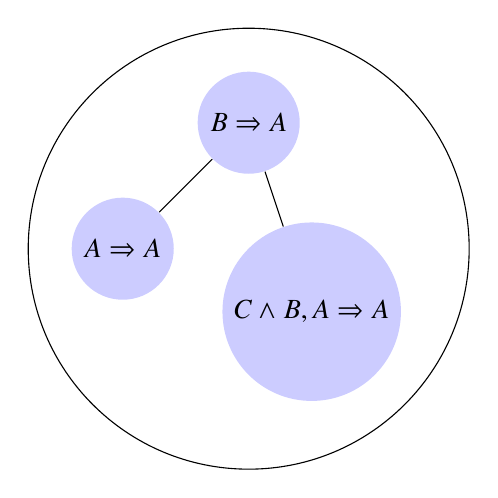
\begin{tikzpicture}
[scale=.8,auto=left,every node/.style={circle,fill=blue!20}]
\draw (3,3) circle (3.5);
\node (n1) at (1,3) {$A \Rightarrow A$};
\node (n2) at (3,5) {$B \Rightarrow A$};
\node (n3) at (4,2)  {$C \wedge B, A \Rightarrow A$};
\foreach \from/\to in {n1/n2,n2/n3}
\draw (\from) -- (\to);

\end{tikzpicture}


, if
 If $C$ $I(\Gamma \Rightarrow A)=1$ then
so does $I(\Pi, \Box \Gamma \Rightarrow \Box A, \Delta) = 1$ for example:
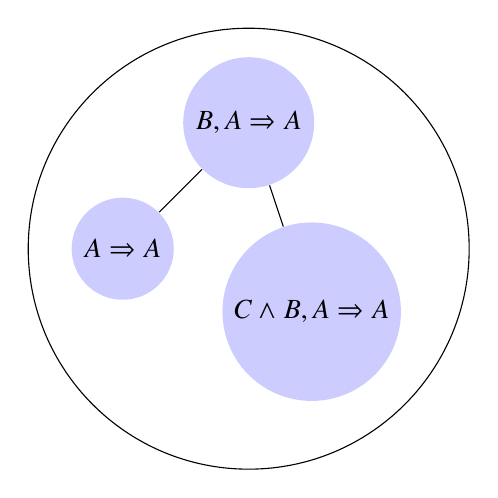
\begin{tikzpicture}
[scale=.8,auto=left,every node/.style={circle,fill=blue!20}]
\draw (3,3) circle (3.5);
\node (n1) at (1,3) {$A \Rightarrow A$};
\node (n2) at (3,5) {$B, A \Rightarrow A$};
\node (n3) at (4,2)  {$C \wedge B, A \Rightarrow A$};
\foreach \from/\to in {n1/n2,n2/n3}
\draw (\from) -- (\to);

\end{tikzpicture}

Therefore $R_k$ is sound.

% I just don't know how to explain this crap.

\section{}
\subsection{Prove $\Box p \Rightarrow \Box \Box p$}
Prove that the sequent $\Box p \Rightarrow \Box \Box p$, where $p$ is a
propositional variable, is not derivable in $GKC_k$.

A propositional variable is either true or false (boolean). To prove
$\Box p \Rightarrow \Box \Box p$ is not derivable in $GKC_k$ we assume
it is derivable and try to construct a prove towards it from the axioms.

The Ax ($\Gamma, A \Rightarrow A \Delta$) Axiom cannot be used because it
doesn not contain propositional vraibles. So we're left with the
$L\bot(\Gamma, \bot \Rightarrow \Delta)$ and $R\top(\Gamma \top
\Rightarrow \Delta)$ axioms
\subsubsection{$L\bot$}
$(\Gamma, \bot \Rightarrow \bot, \Delta)$ will be used as starting point
because it is a valid axiom, and the p needs to be on both sides.
\begin{prooftree}
	\AxiomC{$\Gamma, \bot \Rightarrow \bot, \Delta$}
	\RightLabel{$R_k$}
	\UnaryInfC{$\Gamma, \Box \bot \Rightarrow \Box \bot, \Delta$}
\end{prooftree}
There are after this point however no rules available to add a single box
on 1 side, so the $L\bot$ axiom can't be used to derive
\subsubsection{$L\top$}
$(\Gamma, \top \Rightarrow \top, \Delta)$ will be used as starting point
because it is a valid axiom, and the p needs to be on toph sides.
\begin{prooftree}
	\AxiomC{$\Gamma, \top \Rightarrow \top, \Delta$}
	\RightLabel{$R_k$}
	\UnaryInfC{$\Gamma, \Box \top \Rightarrow \Box \top, \Delta$}
\end{prooftree}
There are after this point however no rules available to add a single box
on 1 side, so the $L\top$ axiom can't be used to derive
$\Box p \Rightarrow \Box \Box p$

\subsubsection{Conclusion}
Because there are no axioms available for the sequent
($\Box p \Rightarrow \Box \Box p$) to work towards, it has been
proven that the sequant is not derivable.

\subsection{Prove $\Box A \to \Box \Box A$ }
Prove that $\Box A \to \Box \Box A$ holds in all transitive Kripke models.

Transitivity means $uRw$ and $vRw$ then $uRw$. So if $\Box A$, A is in every
state. Thus you know that every state is accessible to another state because
its transitive. So you can say $\Box \Box A$

\subsection{Explain why 2.1 and 2.2 imply incompletness}
Explain why 2a and 2b imply that K is not complete with respect to
transitive Kripke models.

Becasue if you create a sequent of 2.2 like this:
$\Rightarrow \Box A \to \Box \Box A$ and apply the $L\to$ opperation,
the formula is essentlially the same as 2.1. But in 2.1 we've shown
that the formula is *not* derivable. So we have some semantic which is
true but a system that says its not true, which indicates incompleteness.

\section{Prove, for any propositional}
Let G denote the calculus GKC extended by the rule
\begin{prooftree}
	\AxiomC{$\Box \Gamma, \Gamma \Rightarrow A$}
	\RightLabel{$R$}
	\UnaryInfC{$\Box \Gamma \Rightarrow \Box A$}
\end{prooftree}
\subsection{Prove p}
Prove, for any propositional variable $p$,
that $\Box p \Rightarrow \Box \Box p$ is not provable in G.

The Ax ($\Gamma, A \Rightarrow A \Delta$) Axiom cannot be used because it
doesn not contain propositional vraibles. So we're left with the
$L\bot(\Gamma, \bot \Rightarrow \Delta)$ and $R\top(\Gamma \top
\Rightarrow \Delta)$ axioms
\subsubsection{$L\top$}
$(\Gamma, \top \Rightarrow \top, \Delta)$ will be used as starting point
because it is a valid axiom, and the p needs to be on toph sides.
\begin{prooftree}
	\AxiomC{}
	\RightLabel{$L\top$}
	\UnaryInfC{$\Box \Box \top, \Box \top, \top \Rightarrow \top$}
	\RightLabel{$R$}
	\UnaryInfC{$\Box \Box \top, \Box \top\Rightarrow \Box \top$}
	\RightLabel{$R$}
	\UnaryInfC{$\Box \Box \top\Rightarrow \Box \Box \top$}
\end{prooftree}
There are after this point however no rules available to remove a single box
on the left side, so the $L\top$ axiom can't be used to derive
$\Box p \Rightarrow \Box \Box p$.

\subsubsection{$L\bot$}
$(\Gamma, \bot \Rightarrow \bot, \Delta)$ will be used as starting point
because it is a valid axiom, and the p needs to be on both sides.
\begin{prooftree}
	\AxiomC{}
	\RightLabel{$L\bot$}
	\UnaryInfC{$\Box \Box \bot, \Box \bot, \bot \Rightarrow \bot$}
	\RightLabel{$R$}
	\UnaryInfC{$\Box \Box \bot, \Box \bot\Rightarrow \Box \bot$}
	\RightLabel{$R$}
	\UnaryInfC{$\Box \Box \bot\Rightarrow \Box \Box \bot$}
\end{prooftree}
There are after this point however no rules available to remove a single box
on the left side, so the $L\bot$ axiom can't be used to derive
$\Box p \Rightarrow \Box \Box p$.

\subsubsection{Conclusion}
Because there are no axioms available for the sequent
($\Box p \Rightarrow \Box \Box p$) to work towards, it has been
proven that the sequant is not derivable.

\subsection{Prove s from $GKC_{K4}$ in $G$}
Prove that not every sequent provable in $GKC_{K4}$
is provable in G.

To proof this one sequent will be shown to be provable in $GKC_{K4}$
and then will be shown this sequant is not provable in $G$

G = GKC and:
\begin{prooftree}
	\AxiomC{$\Box \Gamma, \Gamma \Rightarrow A$}
	\RightLabel{$R$}
	\UnaryInfC{$\Box \Gamma \Rightarrow \Box A$}
\end{prooftree}

$GKC_{K4}$ = GKC and:
\begin{prooftree}
	\AxiomC{$\Box \Gamma, \Gamma \Rightarrow A$}
	\RightLabel{$R$}
	\UnaryInfC{$\Pi, \Box \Gamma \Rightarrow \Box A, \Delta$}
\end{prooftree}

As an intial observation the rules of $GKC_{K4}$ and $G$ are functionally
the same. They're both intendid to remove the box on the right side and to
hide it away in the left side in one of the `garbage' spots $(\Pi$ and 
$\Delta)$ of the axioms.

However the $GKC_{K4}$ has also garbage spots in the conclusion. So to show
something is proofable in $GKC_{K4}$ and not in $G$ all you need to do is
fill in one of those garbage spots. Consider the following sequant:

\[A, \Box B \Rightarrow \Box B, A\]

This can be solved in $GKC_{K4}$ in the following way:

\begin{prooftree}
	\AxiomC{}
	\RightLabel{Ax}
	\UnaryInfC{$\Box B, B \Rightarrow B$}
	\RightLabel{$R$}
	\UnaryInfC{$A, \Box B \Rightarrow \Box B, A$}
\end{prooftree}

However this sequant is not solvable in G, the rule for dealing with the 
boxes cannot match the `garbage'

\subsection{Does the converse hold?}
yes because the `garbage' spots are allowed to be empty.
%Yes or no, maybe a because
\section{Prove, using soundness}
Prove using soundness, that $GKC_K$ does not derive $(\Box A \Rightarrow A)$.

$(\Box A \Rightarrow A)$ can't be derived in $GKC_K$ because
$(\Box A \Rightarrow A)$ isn't valid in kripke. $\Box A$ inidicates that the
state should be able to get to A. But it does not mean that the current
state has an $A$ as this sequance indicates. So $(\Box A \Rightarrow A)$
shouldn't be derivable in $GKC_K$ otherwise $GKC_K$ wouldn't be sound.
This is what thad to be shown.

\section{Prove, that if $\vdash_{GKC_K}$}

Prove that if $\vdash_{GKC_K}(\Rightarrow \Box A)$, then
$\vdash_{GKC_K}(\Rightarrow A)$

\end{document}
